
%(BEGIN_QUESTION)
% Copyright 2014, Tony R. Kuphaldt, released under the Creative Commons Attribution License (v 1.0)
% This means you may do almost anything with this work of mine, so long as you give me proper credit

Suppose you were designing a circuit that required two LEDs for ``power on'' indication.  The power supply voltage is 15 volts, and each LED is rated at 1.6 volts and 20 mA.  Calculate the dropping resistor sizes and power ratings:
Du skal beregne verdien som motstandene må ha i denne kretsen for at lysdiodene skal få rett strøm. Tilførselsspenningen er 15 V og lysdiodene er opptitt til 1.6V og 20mA. 

Regn også ut hvor stor effekt motstandene må tåle. 

$$\includegraphics[width=8cm]{i01170x01.eps}$$

Etter at du har gjort dette, fårslår en kollega at du kan bruke en felles motstand for diodene. Dette gir jo en krets med mindre komponenter. 

$$\includegraphics[width=8cm]{i01170x02.eps}$$

Beregn verdi og effekt for den nye motstanden. 


\underbar{file i01170}
%(END_QUESTION)





%(BEGIN_ANSWER)

With two resistors: $R_1 = R_2 = 670 \> \Omega$, rated for at least 0.268 watts (1/2 watt would be a practical rating). 

\vskip 10pt

With one resistor: $R_1 = 335 \> \Omega$, rated for at least 0.536 watts (1 watt would be a practical rating). 

%(END_ANSWER)





%(BEGIN_NOTES)

If students are not yet familiar with the ``+V'' symbol used to denote the positive power supply connection in this schematic, let them know that this is a very common practice in electronic notation, just as it is common to use the ground symbol as a power supply connection symbol.

The follow-up question is a very practical one, for it is seldom that you have the exact components on-hand to match the requirements of a circuit you are building.  It is important to understand which way is safer to err (too large or too small) when doing ``as-built'' design work.

%INDEX% Electronics review: series-parallel circuits

%(END_NOTES)


